\section{Energetic particles in the heliosphere}
\label{sec:particles_heliosphere}


The heliosphere is a vast, bubble-like region in space that envelops the Sun. This region is moving with respect to the \ac{ISM} with a speed of about 25 km/s \citep{McComas2015ApJS}. It is also a plasma cavity that is created by the Sun and is governd by the solar wind and its magnetic field; a substantial amount of plasmas of various particle populations fill this space. The particle populations are identified from Fig.\ref{Fig:Oxygen_spectra_heliosphere} which is adapted from \citet{Mewaldt-2001}. Based on the accumulated measurements of oxygen by the \ac{ACE} between 1997 and 2000 at 1 au, the oxygen fluence spectrum which spans over more than seven orders of magnitude from keV/nuc to GeV/nuc provides clear insight into the lower energy particles including the slow solar wind, the fast solar wind, the suprathermal tails, and high energetic particles composed of \acp{SEP}, \acp{ACR}, and the extremely high energetic \acp{GCR}. 

%Among them \acp{GCR} originate from distant sources outside the solar system, while \acs{ACR} sources are located near the boundary of the heliosphere. The remaining energetic particles are accelerated and generated inside of the heliosphere at the multiple locations, including the solar surface, interplanetary space and even the planets, for instance Jupiter.

\begin{figure}
	% moving the figure to the second page
	\centering
	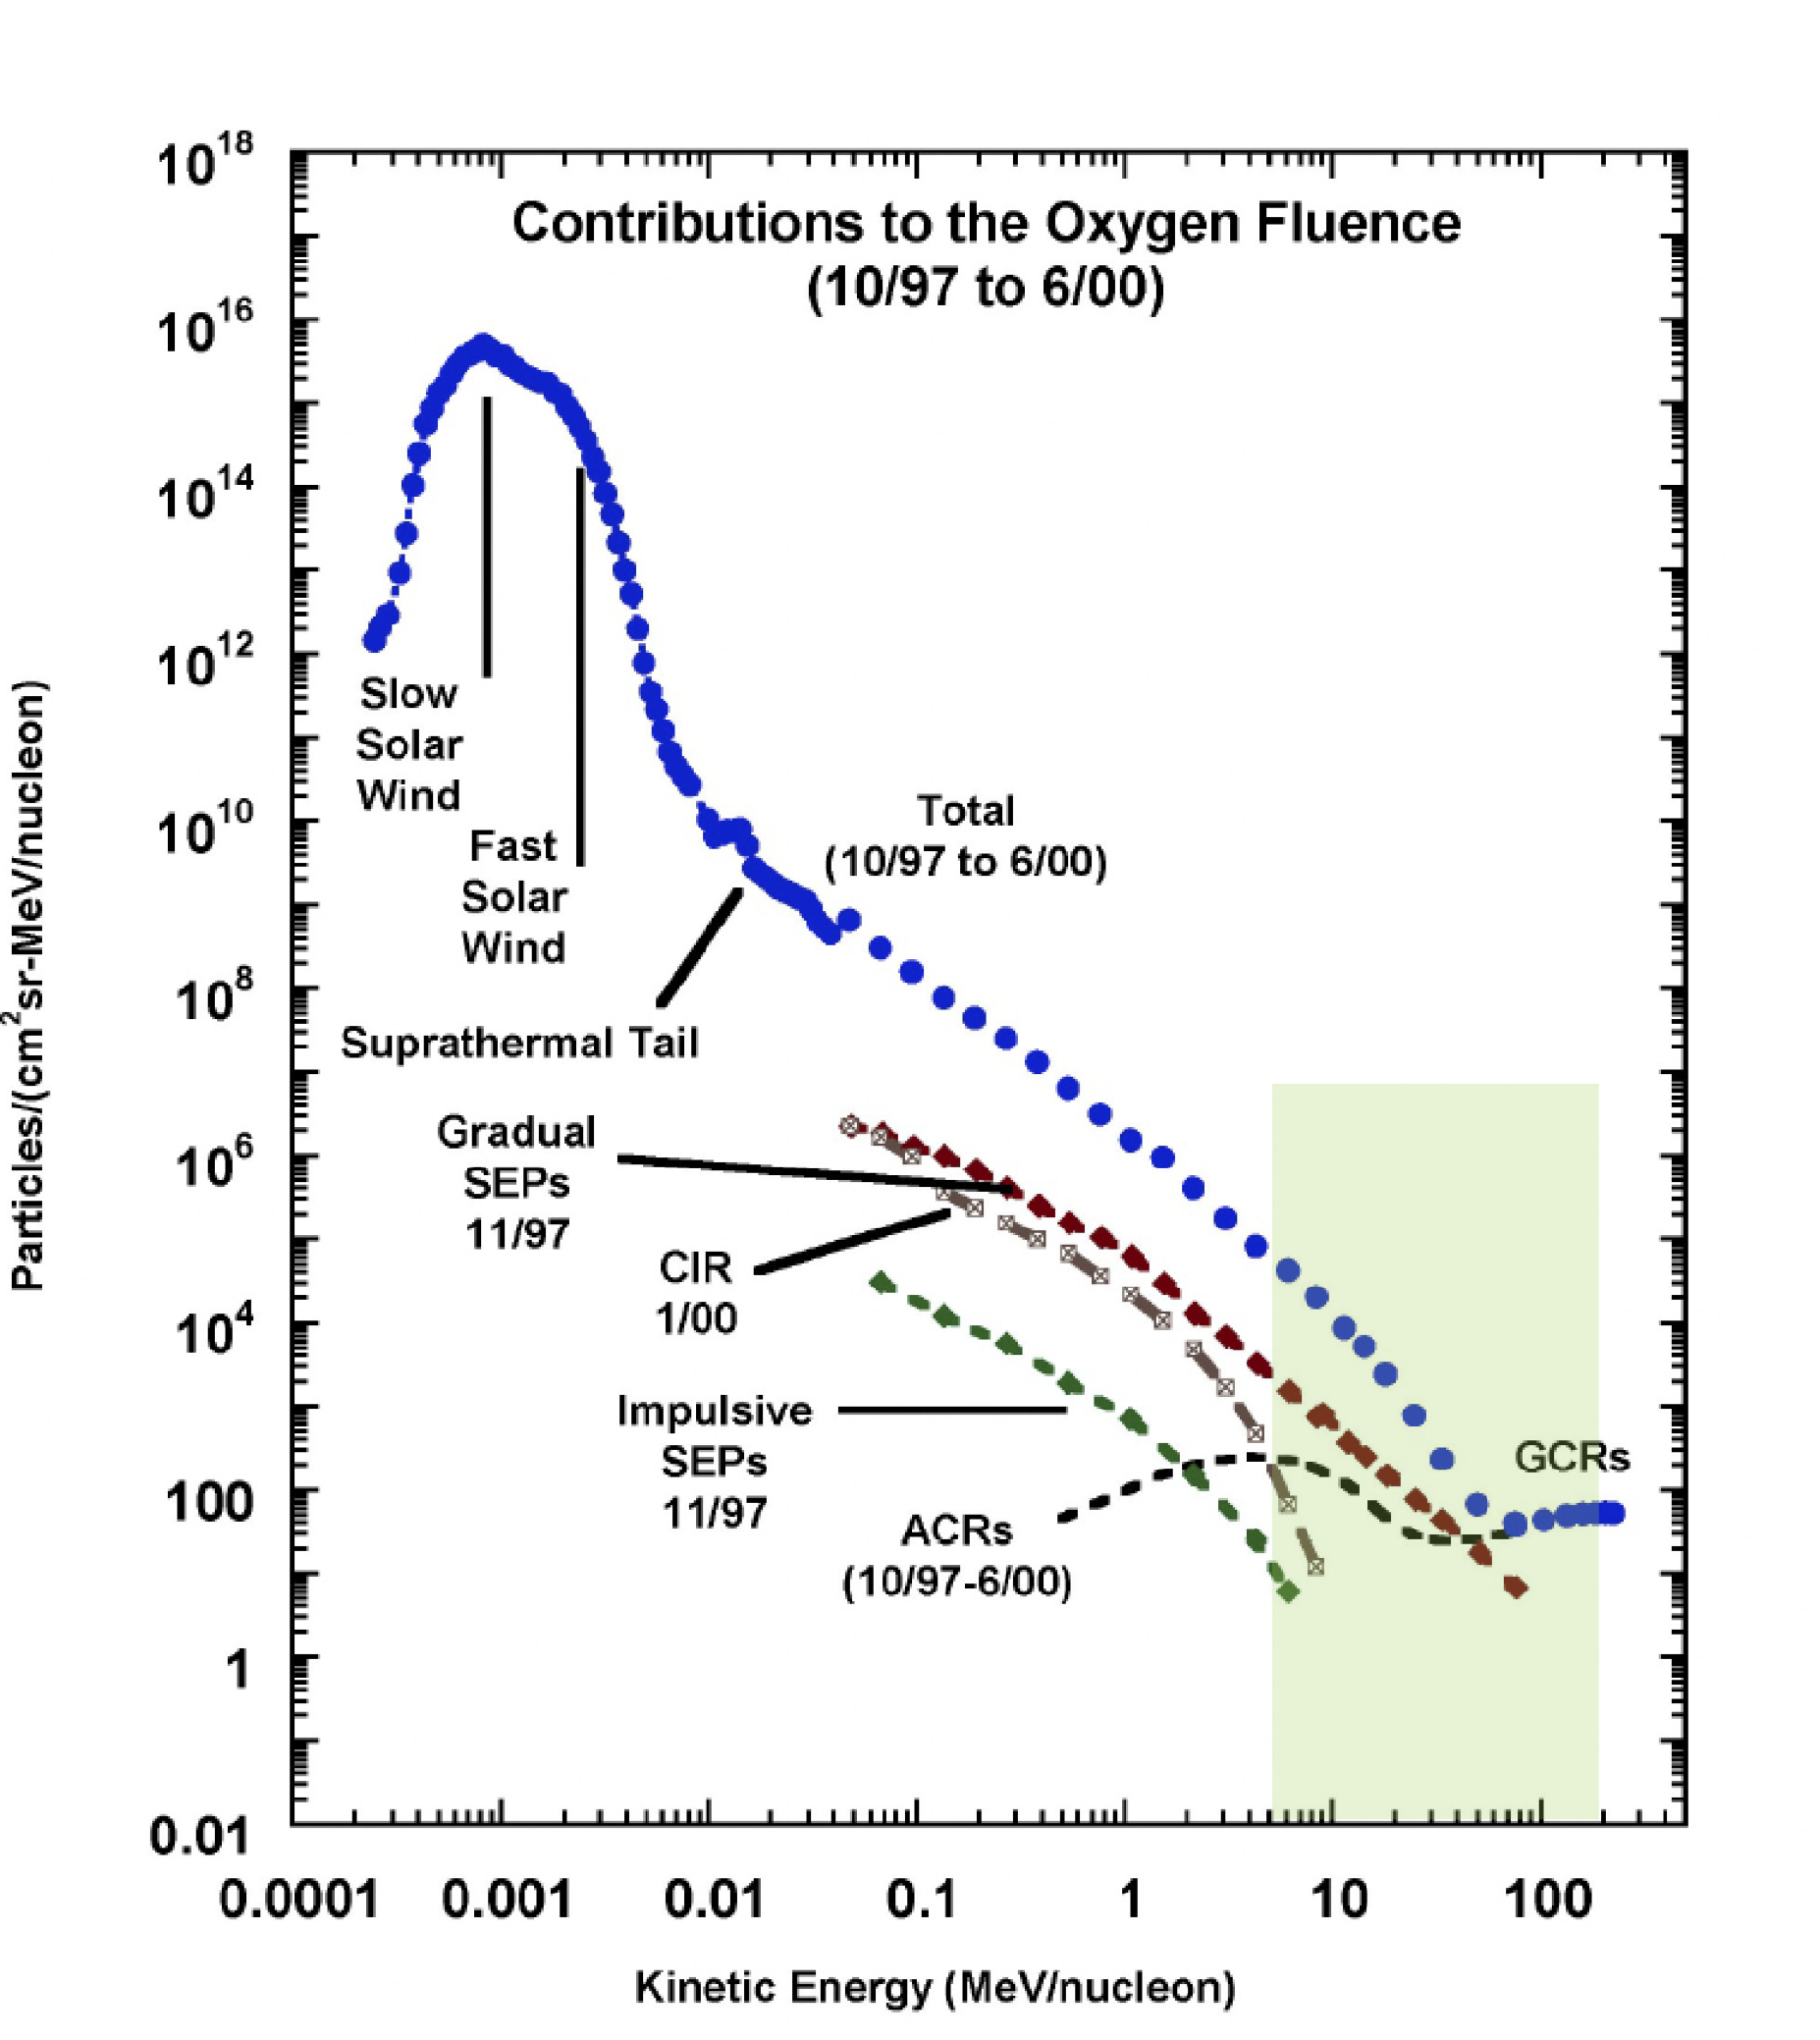
\includegraphics[width = 0.8\textwidth]{images/heliospheric_particle_spectra_color.png}
	\caption[Energy spectra of oxygen ions in near-Earth space]{The typical oxygen spectra in the interplanetary space near Earth, indicating the contributions of different particle populations, particularly in the energy range between few MeV/nuc and few hundreds MeV/nuc (green shaded region), where \acs{SEP}, \acs{ACR} and \acs{GCR} coexist. The spectra of other particle species such as, helium and protons have a similar shape but a different flux level in the corresponding energy regime. The figure is adapted from \citep{Mewaldt-2001}}
	\label{Fig:Oxygen_spectra_heliosphere}
\end{figure}


The solar wind is a stream of charged particles released from the solar corona, the upper atmosphere of the Sun. This plasma consists of mainly protons and electrons that continously flow outward and expand to about $\sim$ 100 au (depending on the direction and the phase of solar activity cycle). The typical energy range of the solar wind is between 0.5 keV and 4.5 keV. Depending on the locations that produce the solar wind, the speed and density of the solar wind might be different. For instance the fast solar wind with a typical speed between 500 and 800 kilometers per second is emitted from the coronal holes which are funnel-like regions of open field lines in the magnetic field and usually appear at the north and south pole of the Sun \citep{Sakao2007, Tu2005, hundhausen1968state}. Therefore, the fast solar wind dominates the high latitude regions. On the other hand, the slow solar wind is observed to have a velocity of about 300 - 500 kilometers per second and is believed to originate from the streamer belt along the equatorial belt. The slow solar wind is more likely to be observed in the low latitude regions.


%plasma embedding with magnetic field

Suprathermal particles are charged ions and electrons that move about two to hundreds times faster than the solar wind particles. In the spectrum shown in Fig.\ref{Fig:Oxygen_spectra_heliosphere}, the suprathermal particles are beyond the tails of the fast solar wind and are the dominant particle population between few keV to hundreds of keV. The source of the suprathermal particle might be accelerated solar wind and the remanent of the previous solar eruptions and \ac{SEP} events \citep{Gloeckler1995SSRv}. Suprathermal particles are suspected to play an important role as seed particles for \ac{SEP} events \citep{Kahler2019ApJ}.
%Those particles play an important role in contributing seed particles for \ac{SEP} events.

Above the energy of suprathermal particle is the energy range that we are interested in this thesis, especially the energy range between 10 MeV/nuc and few hundred MeV/nuc where the dominant particles are \acp{SEP} (not limited to this energy range), \acp{ACR} (up to $\sim$ 100 MeV/nuc) and lower energy \acp{GCR}. The measurements we used in this study are from this energy range.

\acp{SEP} are high energetic particles with energy of few keV up to $\sim$ GeV originated from the sun and are accelerated by solar flares and \ac{CME}-driven shocks. \acs{SEP} events are intermittent, short term, and normally intensive, compared with cosmic rays \citep{Reames1999}. Different type of \acs{SEP} events persist for different time scales from few hours to few days. Such high energy particles are one of the major threats in the space.
%also particle from solar, accelerated by different mechanism. The enery range of \ac{SEP} are quite broad, especially depending the on where the measurement carried on. Recently \ac{SOLO} and \ac{PSP} frequently measure the hundreds keV \ac{SEP}.

\acs{ACR} are believe to be the high energy interstellar pick-up ions \citep{Giacalone2022SSRv} which are ionized neutral interstellar atoms generated by solar UV radiation after neutral atoms move cross the boundary and enter the heliosphere. Those ionized particle are then carried by the expanding solar wind to the outer boundary of the helioesphere, where they are accelerated by the termination shock and then propagate inwards. The typcial \ac{ACR} species that have been observed are proton, helium, oxygen, nitrogen, iron and neon. 

\acp{GCR} are the fully ionized particles that are accelerated at the so-called supernova remnants \citep{Blasi2013AARv2013} outside of the solar system. Those high energy particles bombard Earth in a constant and slowly varying way. The complete GCR spectrum cover the energy from typical 1MeV \citep{Potgieter2013LRSP} to ZeV which is larger than the energy range in Fig.~\ref{Fig:Oxygen_spectra_heliosphere}. \acp{GCR} are comprised of about 89\% of hydrogen, 10\% of helium, 1\% of heavier ions as well as electrons, positrons and antiprotons. 

After entering the heliosphere, the transport of both \acp{ACR} and \acp{GCR} are controled by the \ac{HMF}, hence \ac{ACR}'s and \ac{GCR}'s temporal variaton is highly related to the solar activity and solar modulation, which periodically changes in 11 and 22 year periods. 


% LND and SOLO/EPD are new instruments;

% In the helioshphere, 

% Questions:


% 0. Cross calibrate the new data from new instrument; how is the performance of the new instrument? Are they good enough? - To answer this question
% 1. How the widespread SEP generated



\section{Motivation}

\todo[options]{
	- motivate the topic of your thesis, explain why this is something interesting to work on 
- discuss what questions your thesis aims to address
- provide an overview on how these questions have been addressed in the preexisting literature, and explain how and why you work is necessary/ relevant to contribute to this. 
- optioannly give an overview on the structure of the thesis.
}
 

% questions:
% motivation to study radiation envirnoments:

% overview on the structure of the thesis
% the following we already talked about on Friday:

% From my point of view, Chapter 1 here is not the "introductiion" but the theoretical background.

% From my point of view, the introduction should 
% - motivate the topic of your thesis, explain why this is something interesting to work on 
% - discuss what questions your thesis aims to address
% - provide an overview on how these questions have been addressed in the preexisting literature, and explain how and why you work is necessary/ relevant to contribute to this. 
% - optioannly give an overview on the structure of the thesis. 

% A dateiled discussion/ overview on the thereitical background should then (from my point of view come in the next chapter)


% What is the motivation to study radiation envirnoments at all? (this should be included/ pointed out as part of the motivation in the introduction)

% Why are the three points ordered in this way?

% From the papers I would expect that: understanding ACR transport (which is imprortant because of ...) is also part of the motivation for your thesis ;

% If you can be more specifiv in the motivation, the better:
% what is the motivation for your research questions? 

% The interesting new solar cycle, the exiciting new missions and the opportunities for multispacecraft observations are all relevant, bu they don;t yet answer:
% - why are these missions (including SOlO and LND) so exciting?
% - what new questions can multipoint measurements address? which of these are you interested in? (what other questions are other people working on with multipoint observations?)
% - what makes Mars and Moon particularly interesting radiation environments?
% Future colony, human activity, astronauts

% -why is it interesting that the current solar cycle is nusual (and how can yout thesis contribute to that)?
%  The unusual solar cycle 

The inspiration of this thesis arises from the following three aspects:
\begin{itemize}
	\item New missions and new measurements:
	%Over the last few years, several thrilling missions have been successfully launched after extensive preparation, such as \ac{PSP}, \ac{SolO}, \ac{Bepi}, lunar mission like the Chang'E series mission, \ac{ESA}'s Jupiter Icy Moons Explorer(Juice),
	% and Chinese missions like CHASE and ASO-S. 
	In this thesis, we focused particularly on the new measurement from \ac{SolO} and the \ac{LND}. The former provides the fantastic oppurtunity to study the solar activity from such a close distance and the latter is the first human mission on the surface of Moon monitoring the radiation environment. The availability of those new observations could enhance our studies of the heliosphere. 
	Once we have the new data from the new instrument, the most fundemental question is how the data looks like in this new instrument.
	%Are they useful? Any new insight shed into the community: validate the instrument performance;
	\item New solar cycle: The recently solar minimum have ended in 2020 with the starti of th new \ac{SC} 25. Many observations haved already implied the unusual quiet property of this solar cycle. The \ac{GCR} flux reached historically high levels in the space age \citep{Fu2021ApJS, Xu2022FrASS}, but ACR intensities are not as high as what , record-setting levels \citet{Strauss2023ApJ}. Moreover, the solar activities raised up rapidly with the onset of \ac{SC} 25 and it could be the strongest \ac{SC} since records began \citep{Nagovitsyn2023SoPh}. The peak of the \ac{SC} might arrive one year earlier than the prediction \textbf{More citation here} \citep{McIntosh2020SoPh}. On the other hand, after the solar activity minimum, the increasing solar eruptions and \ac{SEP} events provide researchers more oppurtunities to study solar activities and their impact on the Earth and planet.
	%Question: How the GCR modulated during the solar minimum? what is the drift and diffusion of ACR looks like in the new cycle?

	\item Multipoint observations in the heliosphere: With the increasing number of missions deployed in space, multipoint observations are becoming more and more important and prevalent, enabling comprehensive moitoring the solar activity at wide spread regions and at different radial distance. %Question: How the wide spread event look like? Any discrepancy between the observation from SOLO and other instruments.
	
\end{itemize}

The structure of the thesis is like this: In next section, we will first introduce the observation and theoretical background of \acp{SEP}, \acp{GCR} and \acp{ACR} in the heliosphere. In Sec.~\ref{chp:instruments}, we will introduce the instruments - \ac{LND} and \ac{SolO}/\ac{HET} - and the data we used in this thesis. Then, we will present observations of the first \ac{SEP} from \ac{LND} in Sec.~\ref{chp:LND_SEP}, \acp{GCR} and secondary protons measured on the lunar surface in Sec.~\ref{chp:LND_GCR_albedo}, quiet time spectra (\ac{GCR}) measured by \ac{SolO} in the inner heliosphere in Sec.~\ref{chp:SOLO_Quite_time} and the \ac{ACR} helium radial gradients in Sec.\ref{chp:ACR_Helium}. The quick summary and outlook will be given in the last section.
In particular, more detailed information of the \ac{LND} are provided in the Appendix ~\ref{chp:LNDinstrument}

% The exploration of space has witnessed a surge in intensity, with an increasing number of countries aspiring to venture into this domain. Noteworthy examples include NASA's initiation of the Artemis mission, which aims to return to the Moon by 2024. Similarly, China has unveiled its plans to establish a lunar base on the lunar surface by the 2030s, while the European Space Agency (ESA) has also embarked on a lunar lander mission. Most recently, a Japanese lunar lander mission was launched; however, it regrettably encountered failure.

% Under these circumstances, the study of solar energetic particles (SEPs) assumes greater significance. SEPs pose a significant radiation hazard for future human exploration on the lunar surface. The most hazardous SEP events have the potential to induce radiation increases of substantial magnitude.

% SEP events directed towards Earth can become an issue of space weather and
% very energetic events can cause a so-called Ground Level Enhancement (GLE).
% This means that the radiation level on the ground increases which can be seen in
% neutron monitor measurements.